\documentclass[oneside, 12pt, letterpaper]{scrreprt}

%%%%%%%%%%%%%%%%%%%%%%%%% Importacion de paquetes y configuraciones %%%%%%%%%%%%%%%%%%%%%%%%%

% Codificación utf8 para colocar símbolos y acentos directamente
\usepackage[utf8]{inputenc}

% Fuente TImes New Roman
\usepackage{times}
\addtokomafont{disposition}{\rmfamily}

% Bibliografia biblio.bib
\usepackage[backend=bibtex, citestyle=authoryear]{biblatex}
\addbibresource{biblio.bib}

% Paquete para el interlineado
\usepackage{setspace}

% Paquete para los margenes
\usepackage[letterpaper]{geometry}

% Márgenes del documento
\geometry{top=30mm,bottom=30mm,left=40mm,right=30mm}

% Cuenta el numero de pagina
\usepackage{lastpage}

% Insertar gráficos
\usepackage{graphicx}

% Colores
\usepackage{xcolor}

% Enlaces en el documento (índice y referencias)
\usepackage{hyperref}

% Enlaces en negro
\hypersetup{
    colorlinks = false,
    linkbordercolor = {white}
}

% Numeración continua para ecuaciones, figuras y tablas 1, 2, 3, 4,... en vez de 1.1, 1.2, 2.1,...
\usepackage{chngcntr}
\counterwithout{figure}{chapter}
\counterwithout{table}{chapter}
\counterwithout{equation}{chapter}

% Paquetes para ayudar a escribir fórmulas matemáticas
\usepackage{amsmath, amsthm, amssymb, amsfonts}

% Paquete que provee \FloatBarrier que permite forzar el posicionamiento de una imagen o tabla
\usepackage{placeins}

% Paquete para formatear los títulos y secciones
\usepackage{titlesec}
\titleformat{\chapter}{\normalfont\large\centering\bfseries}{\MakeUppercase \chaptertitlename \space \Roman{chapter}: \space}{0pt}{\large\MakeUppercase}

% Color codigo python
\usepackage{python_col}

% Idioma
\usepackage[spanish,es-lcroman]{babel}
\selectlanguage{spanish}


%%%%%%%%% Campos de la tesis %%%%%%%%%%%%%%
%% Autor
\newcommand{\autor}{Br. Fulano y Br. Mengano} % Fulano proviene del árabe "fulan" que significa: un tal. Mientras que Mengano viene del árabe "man kan" que significa: quien sea. 
% Título de la tesis
\newcommand{\tesis}{Diseño de una nave espacial para viajes interestelares}
% Profesor
\newcommand{\tutor}{Perencejo}
% Universidad
\newcommand{\universidad}{Universidad de Central de Venezuela}
% Facultad
\newcommand{\facultad}{Facultad de Ingeniería}
% Escuela
\newcommand{\escuela}{Escuela de Ingeniería Mecánica}
% Ciudad
\newcommand{\ciudad}{Caracas}
% Titulo
\newcommand{\titulo}{Ingeniero Mecánico}


%%%%%%%%%%%%%%%%%%%%%%%%% Comienzo del documento %%%%%%%%%%%%%%%%%%%%%%%%%
\begin{document}
% Portada de la tesis titlepage.tex
% Pagina vacía
\thispagestyle{empty}

\begin{center}
	    \changefontsizes{14pt}
		{\normalfont\bfseries \MakeUppercase{Trabajo Especial de Grado}}

	\vspace{9 cm}

        \changefontsizes{14pt}
		{\normalfont\bfseries \MakeUppercase{\tesis}}

\end{center}

\vspace{5cm}

Tutor Académico: \tutor.

\vspace{2cm}
\hspace{6cm}
\begin{minipage}[t]{8.5cm}
       \changefontsizes{12pt} 
		Presentado ante la ilustre \universidad \space por los
		\autor \space para optar al título de \titulo.

\end{minipage}

\vspace{1cm}

\begin{center}
	\ciudad, \the\year
\end{center}


% Interlineado sencillo
\spacing{1}

% Número de pagina
% Numeración romana minúscula (ShareLatex pone Versalitas, no se por qué)
\pagenumbering{roman}
% Comienza en 3 porque se incluye a tapa dura y la contraportada (incluido pero no impreso)
\setcounter{page}{3}
\setcounter{secnumdepth}{0}

% Si hay algo que no aplique comentalo con %
% Dedicatoria dedicatoria.tex
\chapter*{Dedicatoria}
\addcontentsline{toc}{chapter}{Dedicatoria}

Este trabajo esta dedicado ...

% Agradecimientos agradecimientos.tex
\chapter*{Agradecimientos}
\addcontentsline{toc}{chapter}{Agradecimientos}

Este trabajo no habría sido posible sin el apoyo y el estímulo de..

También me gustaría agradecerle a...

No puedo terminar sin agradecer a mi familia...

% Resumen resumen.tex
\addcontentsline{toc}{chapter}{Resumen}

\begin{center}
    % Primer apellido e inicial del segundo y primer nombre e inicial de segundo
    {\normalfont\bfseries Silva P., Juan C. y Pérez R., Luis E.}
\end{center}

\vspace*{\baselineskip}
% titulo de la tesis (no es necesario editar)
\begin{center}
{\changefontsizes{14pt} \normalfont\bfseries \MakeUppercase{\tesis}}
\end{center}

\vspace*{2\baselineskip}

Tutor Académico: \tutor. Tesis. Ciudad, U.C.V. Facultad de Ingeniería. Escuela de Mecánica. \the\year, \pageref{LastPage}.

\vspace*{2\baselineskip}

{\normalfont\bfseries Palabras clave:} Implante metacarpofalángico, Biomecánica, Método de elementos finitos.

\vspace*{2\baselineskip}

{\normalfont\bfseries Resumen.} En el presente Trabajo Especial de Grado se propuso desarrollar un modelo…



% Índice General
\tableofcontents

% Lista de Figuras
\renewcommand{\listfigurename}{Lista de figuras}
\listoffigures

% Lista de tablas
\renewcommand{\listtablename}{Lista de tablas}
\renewcommand{\tablename}{Tabla}
\listoftables

%%%%%%%%%%  Cuerpo del trabajo %%%%%%%%%

% Interlineado 1.5
\spacing{1.5}

% Numeración arábiga desde 1
\clearpage
\setcounter{page}{1}
\pagenumbering{arabic}

% Comienzan las referencias
\begin{refsection}

% Introducción introduccion.tex
\chapter*{Introducción}
\addcontentsline{toc}{chapter}{Introducción}

Los robots son muy importantes en muchas industrias modernas. Los mismos pueden realizar tareas repetitivas, trabajar con grandes cargas, velocidad y precisión...

% Capítulo 1 capitulo1.tex
\chapter{Planteamiento del problema}

\section{El problema}

La manufactura aditiva, también conocida como impresión 3D es una técnica de prototipado rápido que, a pesar de estar en su infancia, está madurando muy rápidamente, con un potencial aparentemente ilimitado. Con su capacidad de reproducir objetos 3D arqueológicos, superficies matemáticas complejas, hasta prótesis médicas, la tecnología tiene un futuro especialmente prometedor para la ciencia, la educación y el desarrollo sostenible (\cite{LowCost3DP}). Incluso algunos autores consideran a esta técnica una revolución en el mundo de la manufactura (\cite{AManufacturingRev}).

\newpage
\section{Objetivos de la investigación}

\subsection{Objetivo General}
Desarrollar un ...

\subsection{Objetivos Específicos}
\begin{itemize}
    \item Estudiar ...
    \item Comparar ...
	\item Realizar ...
	\item Fabricar ...
\end{itemize}

\newpage
\section{Justificación de la investigación}

La investigación tiene como propósito ...

\newpage
\section{Alcances y limitaciones}

\subsection{Alcances}

\begin{itemize}
	\item Alcance 1.
	\item Alcance 2.
	\item Alcance 3.
	\item Alcance 4.
\end{itemize}

\subsection{Limitaciones}

\begin{itemize}
	\item Limitación 1.
	\item Limitación 2.
	\item Limitación 3.
\end{itemize}


% Capítulo 2 capitulo2.tex
\chapter{Marco Teórico}

\section{Antecedentes de la investigación}

En el año 2013, Xuan Song, Yayue Pan y Yong Chen de la University of Southern California publican el articulo “Development of a Low-cost Parallel Kinematic Machine for Multidirectional Additive Manufacturing” en el cual ...

\newpage
\section{Bases teóricas}

\subsection{Manufactura}

La manufactura se puede definir de dos maneras \cite{Groover}: una tecnológica y la otra económica. En el sentido tecnológico, la manufactura es la aplicación de procesos físicos y químicos para alterar la geometría, propiedades o apariencia de un material de inicio dado para fabricar piezas o productos; la manufactura también incluye el ensamble de piezas múltiples para fabricar productos. Los procesos para llevar a cabo la manufactura involucran una combinación de máquinas, herramientas, energía y trabajo manual. En el sentido económico, la manufactura es la transformación de los materiales en artículos de valor mayor por medio de uno o más operaciones de procesamiento o ensamblado. La clave es que la manufactura agrega valor al material cambiando su forma o propiedades, o mediante combinar materiales distintos
también alterados. El material se habrá hecho más valioso por medio de las operaciones de manufactura ejecutadas en él.

\subsection{Tipos de Procesos Aditivos}

Los procesos aditivos incluyen, entre otros, todas las tecnologías de prototipado rápido (Rapid Prototyping) con métodos como la impresión 3D: 

\begin{itemize}
    
    \item Inyección de aglutinante (Binder Jetting).
    \item Fabricación con Filamento Fundido (FFF).
    \item Estereolitografía (SLA).
    \item Sinterizado  Láser Selectivo (SLS). 
    \item Polyjet.
    \item Manufactura por Haz de Electrones (EBM).
    \item 3D Bioprinting.
     
\end{itemize}

\subsubsection{Fabricación con Filamento Fundido (FFF)}

La tecnología que ha popularizado la impresión de figuras y piezas en 3D ha sido la que se conoce como fused feposition fodeling (FDM)...

En la figura \ref{fig2} se puede observar una representación esquemática del proceso FFF donde: 

(a) El material plástico es alimentado desde una bobina a un cabezal móvil  (b) que derrite el plástico y lo extruye. El material (c) es depositado capa por capa en la forma deseada sobre una plataforma (e) que baja después de que cada capa es depositada mientras estructuras de soporte auxiliares desechables (d y f) sirven de andamiaje.   
       
% \FloatBarrier sirve para forzar la ubicación de una imagen o tabla. Se coloca antes y despues de la imagen
%\FloatBarrier
\begin{figure}[htbp!]
    % Centrada
    \centering
    % width=0.5 del ancho de hoja y la imagen FDM.png se encuentra dentro de la carpeta gráficos
    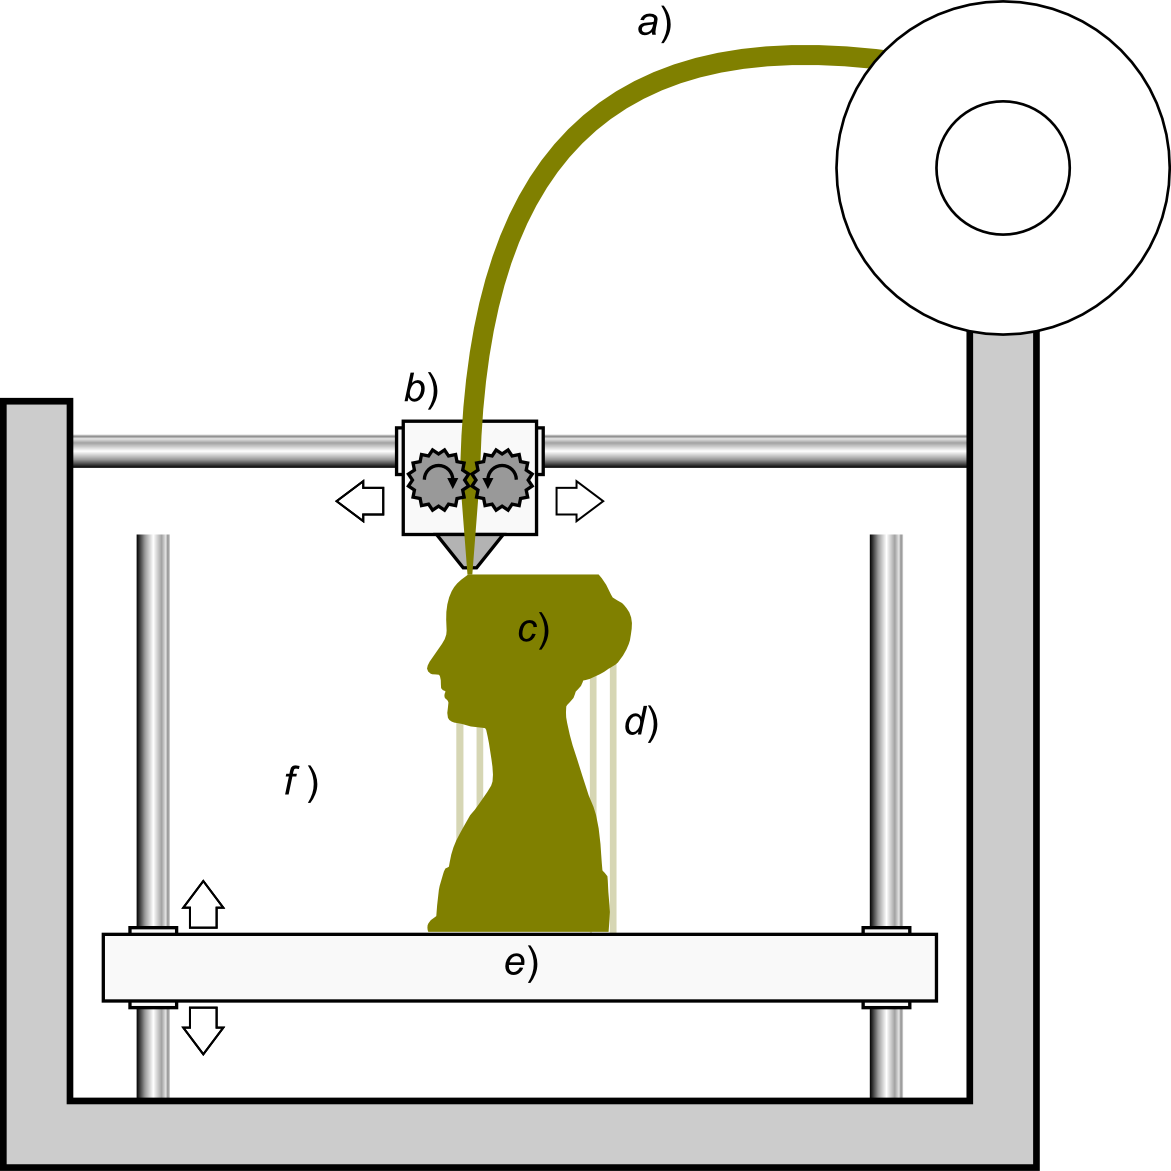
\includegraphics[width=0.5\textwidth]{./graficos/FDM.png}
    % Lo que se muestra debajo
    \caption{Proceso de FFF (Wikipedia).}
    % El alias que le damos para hacer referencia
    \label{fig2}
\end{figure}
%\FloatBarrier

\subsection{Ecuaciones matematicas}

Ecuación centrada y numerada (\ref{eq:ej}):

\begin{equation}\label{eq:ej}
y(x_{i}) = 4 + x_{i}^{2}
\end{equation}

Ecuacion centrada sin numerar 
$$ y(x_{i}) = 4 + x_{i}^{2} $$

Ecuacion en linea $y(x_{i}) = 4 + x_{i}^{2}$, puedes seguir escribiendo.




% Capítulo 3 capitulo3.tex
\chapter{Marco metodológico}

\section{Nivel de la investigación}

Nivel

\newpage
\section{Diseño de la investigación}

Diseño

\newpage
\section{Metodología}

\begin{itemize}
        \item Paso 1.
        \item Paso 2.
        \item Paso 3.
        \item Paso 4.
\end{itemize}

\newpage
\section{Recursos disponibles}

Recursos

%\subsection{Software}

%\begin{itemize}
%        \item Programa 1.
%        \item Programa 2.
%        \item Programa 3.
%        \item Programa 4.
%\end{itemize}

%\subsection{Hardware}
%\begin{itemize}
%        \item Componente 1.
%        \item Componente 2.
%        \item Componente 3.
%        \item Componente 4.
%\end{itemize}

%\subsection{Materiales}
%\begin{itemize}
%        \item Componente 1.
%        \item Componente 2.
%        \item Componente 3.
%        \item Componente 4.
%\end{itemize}

%\subsection{Herramientas}
%\begin{itemize}
%        \item Componente 1.
%        \item Componente 2.
%        \item Componente 3.
%        \item Componente 4.
%\end{itemize}

% Conclusiones conclusiones.tex
\chapter*{Conclusiones}
\addcontentsline{toc}{chapter}{Clonclusiones}

Conclusiones del trabajo

% Recomendaciones recomendaciones.tex
\chapter*{Recomendaciones}
\addcontentsline{toc}{chapter}{Recomendaciones}

% Referencias bibliograficas citadas biblio.bib
% Se cita dentro del documento con \cite{Alias}
\printbibliography[title=Referencias bibliográficas]
\end{refsection}



\nocite{*}
\printbibliography[title=Bibliografías]

\end{document}
